%DO NOT MESS AROUND WITH THE CODE ON THIS PAGE UNLESS YOU %REALLY KNOW WHAT YOU ARE DOING

\chapter{Exercises with Matlab}


\section{ Standard normal distribution } \label{ Standard normal distribution } 
\lstset{language=Matlab,%
    %basicstyle=\color{red},
    basicstyle=\scriptsize,
    breaklines=true,%
    morekeywords={matlab2tikz},
    keywordstyle=\color{blue},%
    morekeywords=[2]{1}, keywordstyle=[2]{\color{black}},
    identifierstyle=\color{black},%
    stringstyle=\color{mylilas},
    commentstyle=\color{mygreen},%
    showstringspaces=false,%without this there will be a symbol in the places where there is a space
    emph=[1]{for,end,break},emphstyle=[1]\color{red}, %some words to emphasise
    %emph=[2]{word1,word2}, emphstyle=[2]{style},    
}
\noindent \textbf{Task:} Now data for four different signal models have to be created. Generate therefore an on [0, 1] uniformly distributed random sequence \texttt{x1} and a standard normal distributed random sequence \texttt{z1,} each with a length of 100 values. Set in both cases first the initial value to 0. Type now these commands in MATLAB in the following order: 
 $$    \texttt{x = x1*5+2;} \quad   \texttt{z = z1*sqrt(0.004);} \quad   \texttt{xy1 = [x exp(1+x*0.6+z)];} $$     
 $$     \texttt{x = x1*4*pi;} \quad  \texttt{z = z1*sqrt(0.05);} \quad  \texttt{xy2 = [x 2*sin(x+1+z)];} $$
 $$    \texttt{x = x1*5;} \quad   \texttt{z = z1;} \quad   \texttt{xy3 =} [\texttt{x} -0.6*\texttt{x}.^3+0.9*\texttt{x}.^2+3*\texttt{x}+4.5+\texttt{z}]; $$
 $$     \texttt{x = x1*5;} \quad   \texttt{z = z1*sqrt(0.004);} \quad \texttt{xy4 =} [\texttt{x} \quad \texttt{exp(0.3+log(x)*0.5+z)}]; $$
 $$   \texttt{x = x1*2*pi;} \quad  \texttt{z = z1*0.5+6;} \quad   \texttt{xy =} [\texttt{z.*cos(x)+4 z.*sin(x)+2}]; $$
 $$   \texttt{save} \quad \texttt{dat3\_1} \quad \texttt{xy1 xy2 xy3 xy4}$$
 $$ \texttt{save} \quad \texttt{dat3\_1} \quad \texttt{xy} $$

\noindent \textbf{Solution:}
\noindent At first, a uniformly distributed random sequence, \texttt{x1} and a standard normal distributed random sequence, \texttt{z1} with length as 100 are created. Then, four different signal models are created using the equations mentioned in the task. The four models are: exponential model, sine model, polynomial model and power model. These models are finally saved in \texttt{dat3\_1}.

\noindent \textbf{MATLAB code:}
\lstinputlisting{assignment3_1.m}
\newpage
\noindent \textbf{Output:}
\noindent The plot of uniform distribution and standard normal distribution is shown in Figure 2.1.
\begin{figure}[H]
    \centering
   \subfloat[Uniform distribution]{ {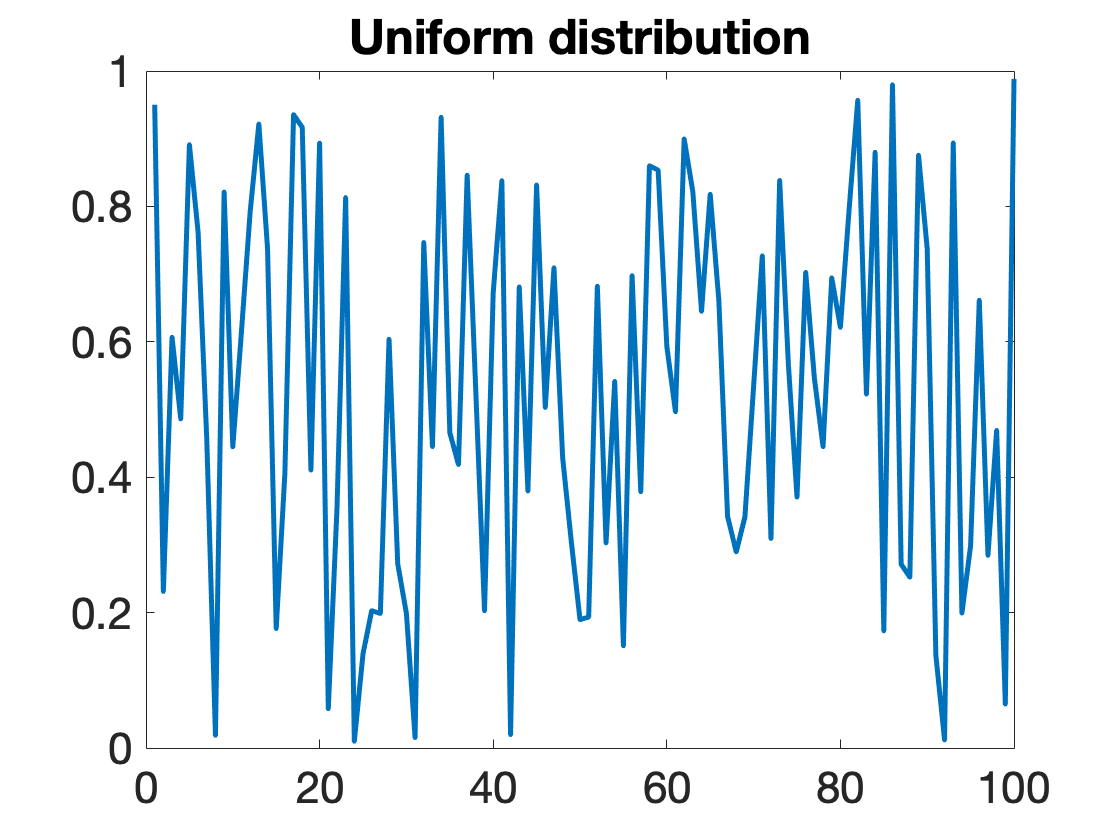
\includegraphics[width=7cm]{ass1_1.png}} }
    \qquad
    \subfloat[Standard normal distribution]{ {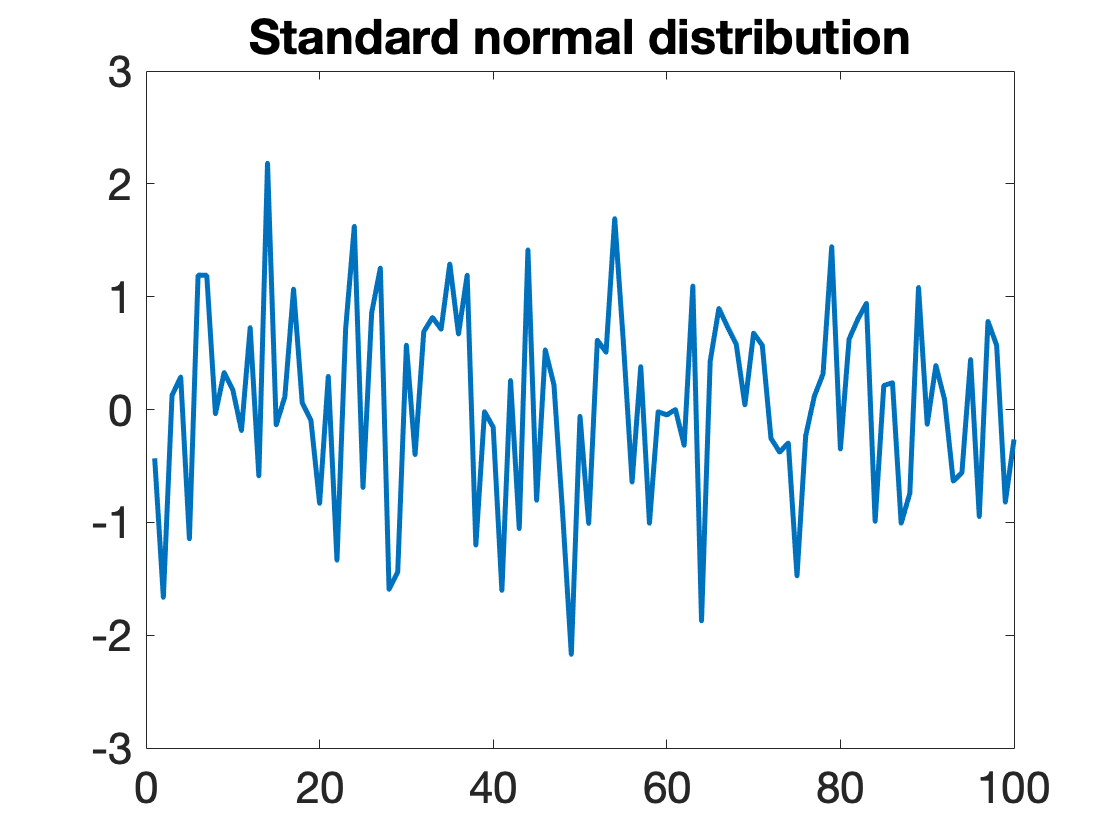
\includegraphics[width=7cm]{ass1_2.png} }}
    \label{fig:example}
    \caption{Distributions}
\end{figure}
\noindent \textbf{Inference:} Four different models which represent exponential, sine, polynomial and power model are created. Also, the uniform distribution with mean as 0 and variance as 1 is generated.
%%%%%%%%%%% code 2 %%%%%


\section{ Model assignment } \label{ Model assignment }
\noindent \textbf{Task:} Load \texttt{dat3\_1} that includes the four 100 x 2 matrices \texttt{xy1, xy2, xy3} and \texttt{xy4.}The two column vectors of each matrix correspond to the observations $x_i$ and $y_i$  of a particular signal model. Show each dataset $x_i$, $y_i$ in a diagram and assign to each matrix a model.
(Note: For the model assignment you can exploit the fact that log $g(x)$ behaves in case of the power model like a logarithmic function while log $g(x)$ depends in case of the exponential model only linearly on $x$.)
 \\

\noindent \textbf{Solution:}
\noindent The four models are first loaded and then are plotted. From the first set of data, i.e., \texttt{xy1}  exponential graph is plotted. And similarly rest of the models are graphed from rest of the data sets. The exponential and power model is also represented using logarithmic Y scale.

\noindent \textbf{MATLAB code:}
\lstinputlisting{assignment3_2.m}

\noindent \textbf{Output:}
\noindent The output after execution of the code is shown in Figure 2.2
\begin{figure}[H]
    \centering
   \subfloat[Exponential model]{ {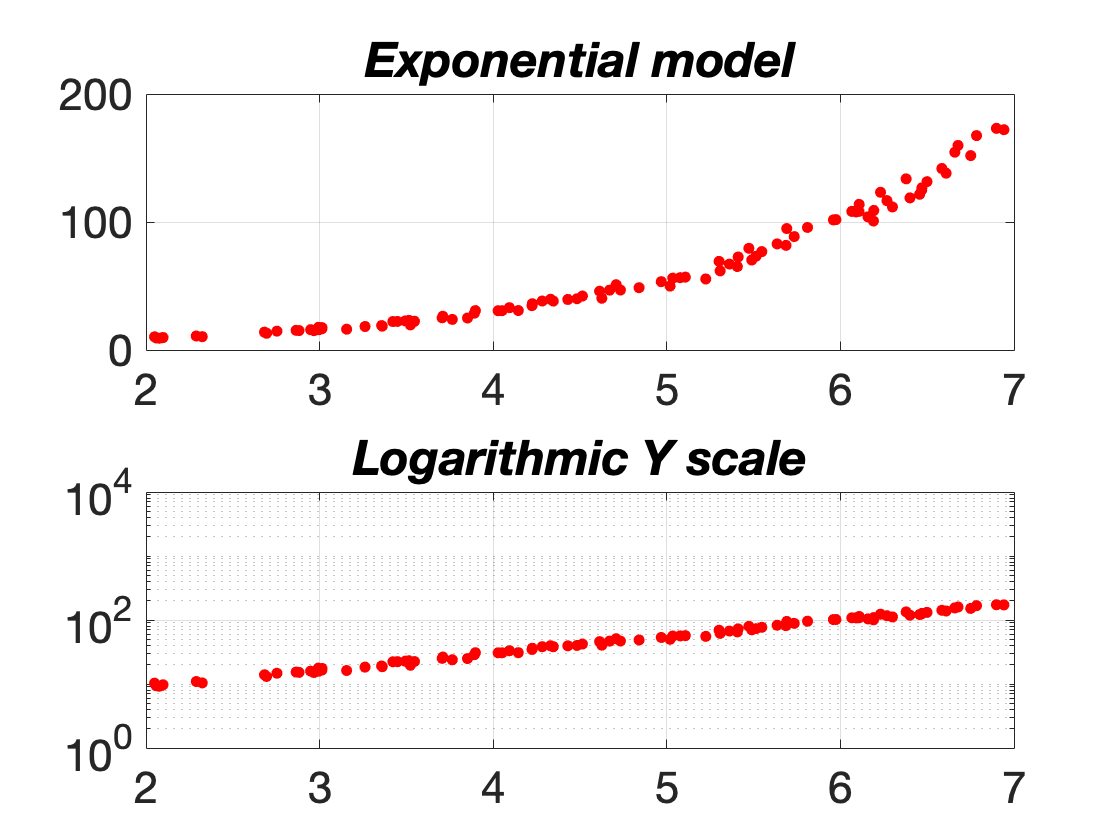
\includegraphics[width=7.2cm]{ass2_1.png}} }
    \qquad
    \subfloat[Sine model]{ {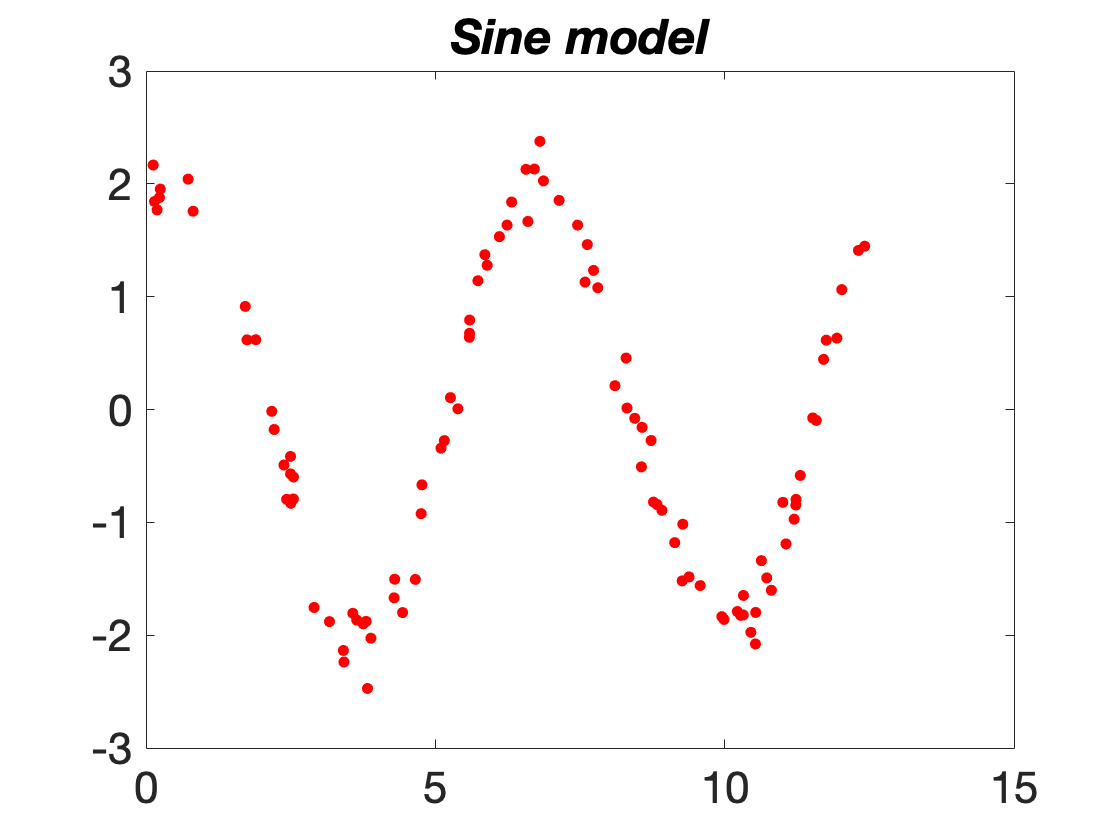
\includegraphics[width=7.2cm]{ass2_2.png} }}
\end{figure}
\begin{figure}[H]
    \centering
   \subfloat[Polynomial model]{ {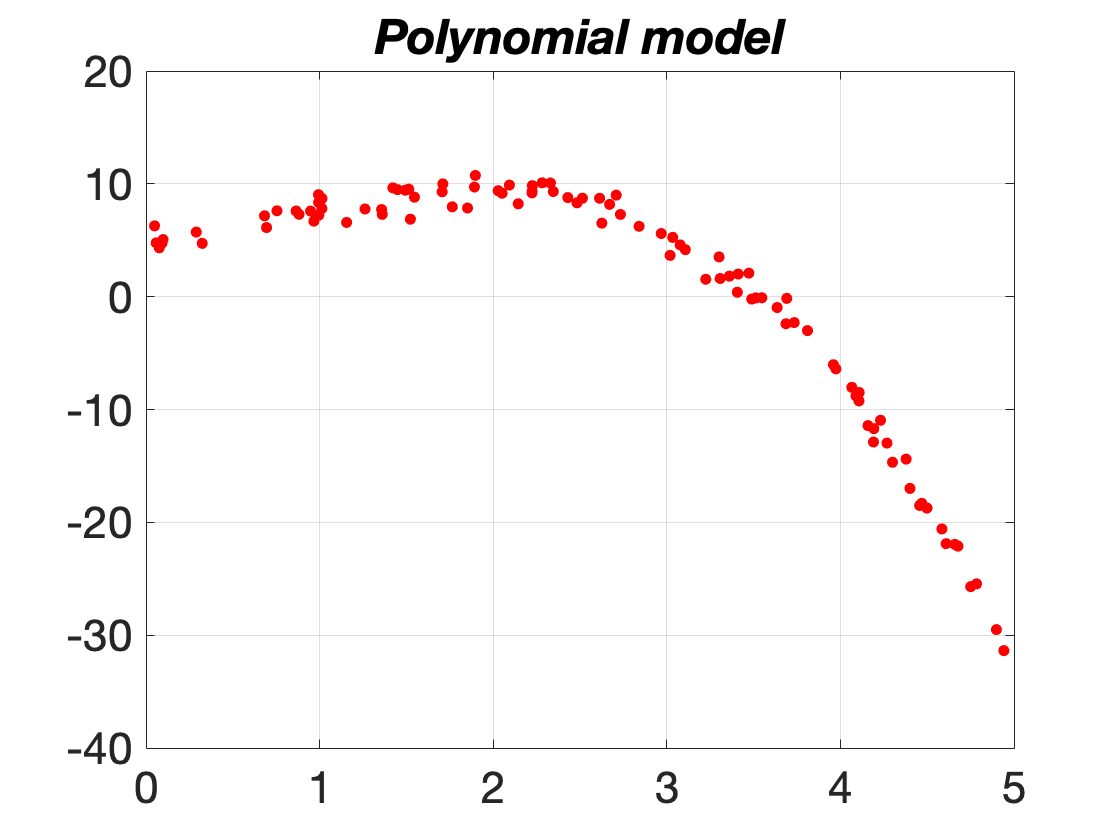
\includegraphics[width=7.2cm]{ass2_3.png}} }
    \qquad
    \subfloat[Power model]{ {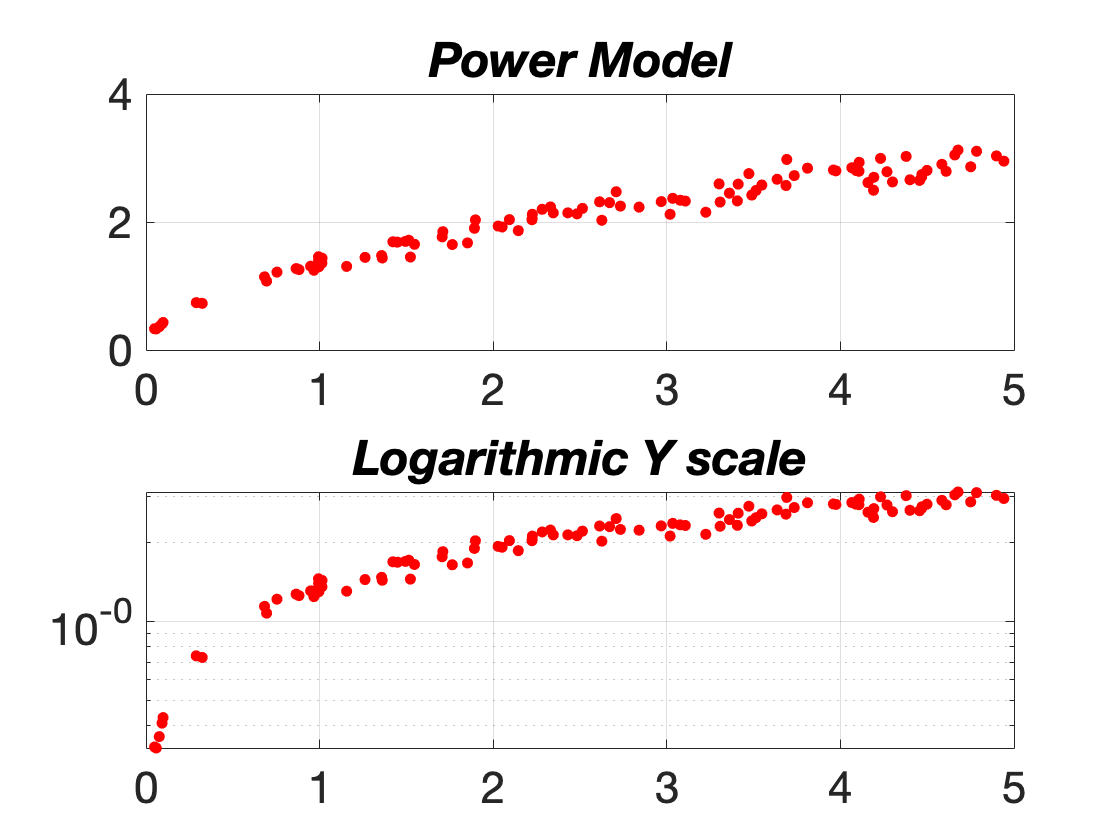
\includegraphics[width=7.2cm]{ass2_4.png} }}
    \caption{Four different models}
\end{figure}

\noindent \textbf{Inference:} We plotted the generated data sets and assigned them a proper model. The logarithm graph of the exponential model is observed to be a straight line because for the exponential model $g(x)$, log($g(x)$) will depend linearly on $x.$ And similarly, for $g(x)$ as a power model, log($g(x)$)  depends logarithmically on $x.$
%%%%%%%%%%%%%%% code 3 %%%%%


\section{ LS-Estimation of different models  } \label{ LS-Estimation of different models }
\noindent \textbf{Task:} Estimate each of the parameter \textit{a, b} and the variance of the measurement errors ${\sigma_z}^2$ of the linearized models, i.e. of the exponential model, the power model and the sine model. Write therefore a function \texttt{LSE} that is able to deal with these three models and with a polynomial model of arbitrary order.

\noindent \textbf{Solution:} We estimate the parameters and the variance of the measurement errors ${\sigma_z}^2$ of the exponential model, the power model, the sine model and the polynomial model. We wrote a function \texttt{LSE} to obtain the above mentioned parameters. The inputs of this function are the data sets from \texttt{dat3\_1} i.e. ($x_i, y_i$), the model whose parameters we want and the integer $p.$ In the case of polynomial model, $p$ represents the order of the polynomial, while for the rest of the model $p = 1.$ We ask the user to input the value of $p$ for the polynomial model.

\noindent \textbf{MATLAB function \texttt{LSE}:}
\lstinputlisting{LSE.m}

\noindent \textbf{MATLAB code:}
\lstinputlisting{assignment3_3.m}

\noindent \textbf{Output:}
\noindent The output after execution of the code is shown below. We gave input as $p = 1$ and $p = 3$. The code prints the parameters for each of the model.
\begin{figure}[H]
    \centering
    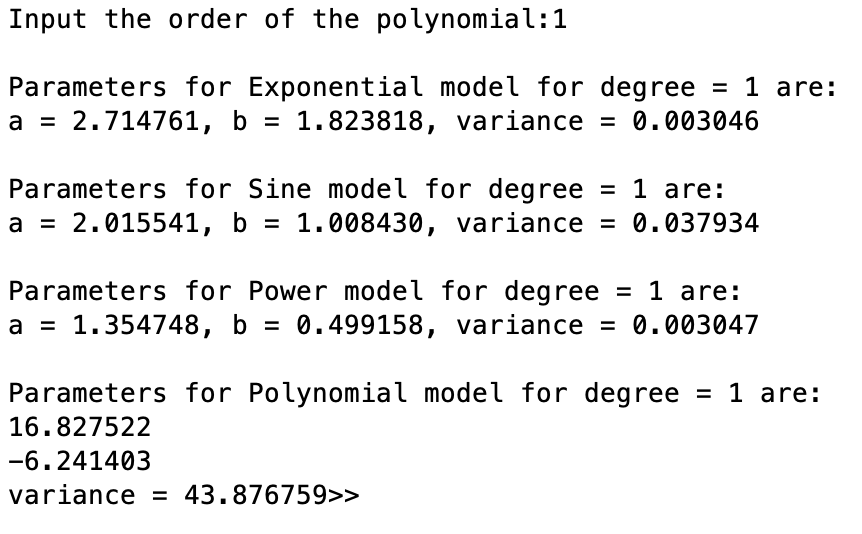
\includegraphics[width=8.3cm]{ass3_2.png}
    \qquad
    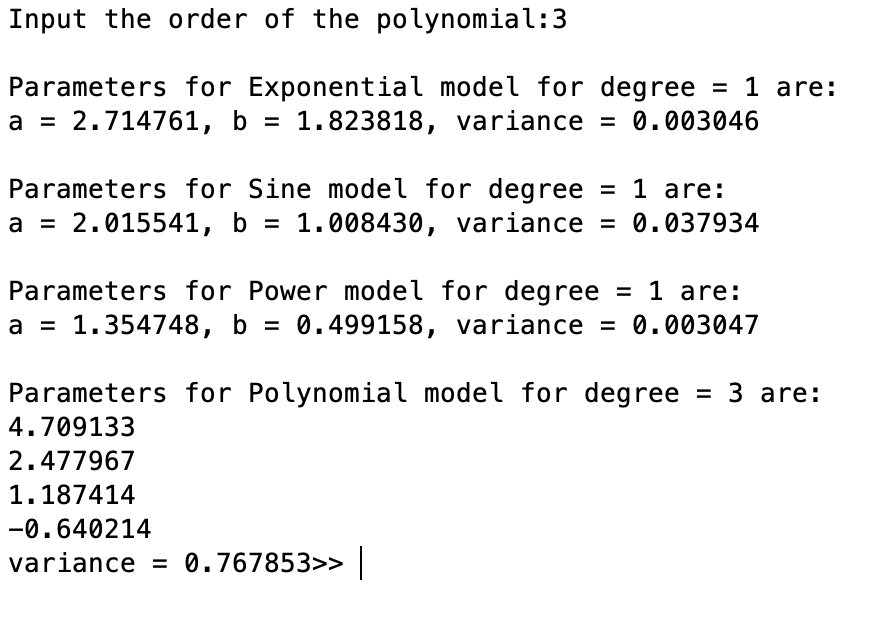
\includegraphics[width=8.3cm]{ass3_1.png} 
\end{figure}

\noindent \textbf{Inference:} Estimation of the wanted parameters for our generated data is done successfully.


%%%%%%%% code 4 %%%%%


\section{ Estimating the order of a polynomial } \label{ Estimating the order of a polynomial}
\noindent \textbf{Task:} Estimate the order $p$ of the polynomial model. Therefore you have to depict the estimated variance versus the model order $p = 1,2,...,10.$ Consider the order that provides the smallest variance as the correct order. Estimate for that order the parameters $a_i$ for $i = 1,2,...,p.$

\noindent \textbf{Solution:} The same function \texttt{LSE} is used to obtain the variance of the polynomial model. The polynomial order $p$, is taken from 1 to 10 and the parameters at each order are shown in the output. 

\noindent \textbf{MATLAB code:}
\lstinputlisting{assignment3_4.m}
\noindent \textbf{Output:} The written code plots variance versus polynomial order. It can be seen that the  variance decreases drastically and after a point it remains constant. The plot can be seen in Figure 2.3.
\begin{figure}[H]
\centering
{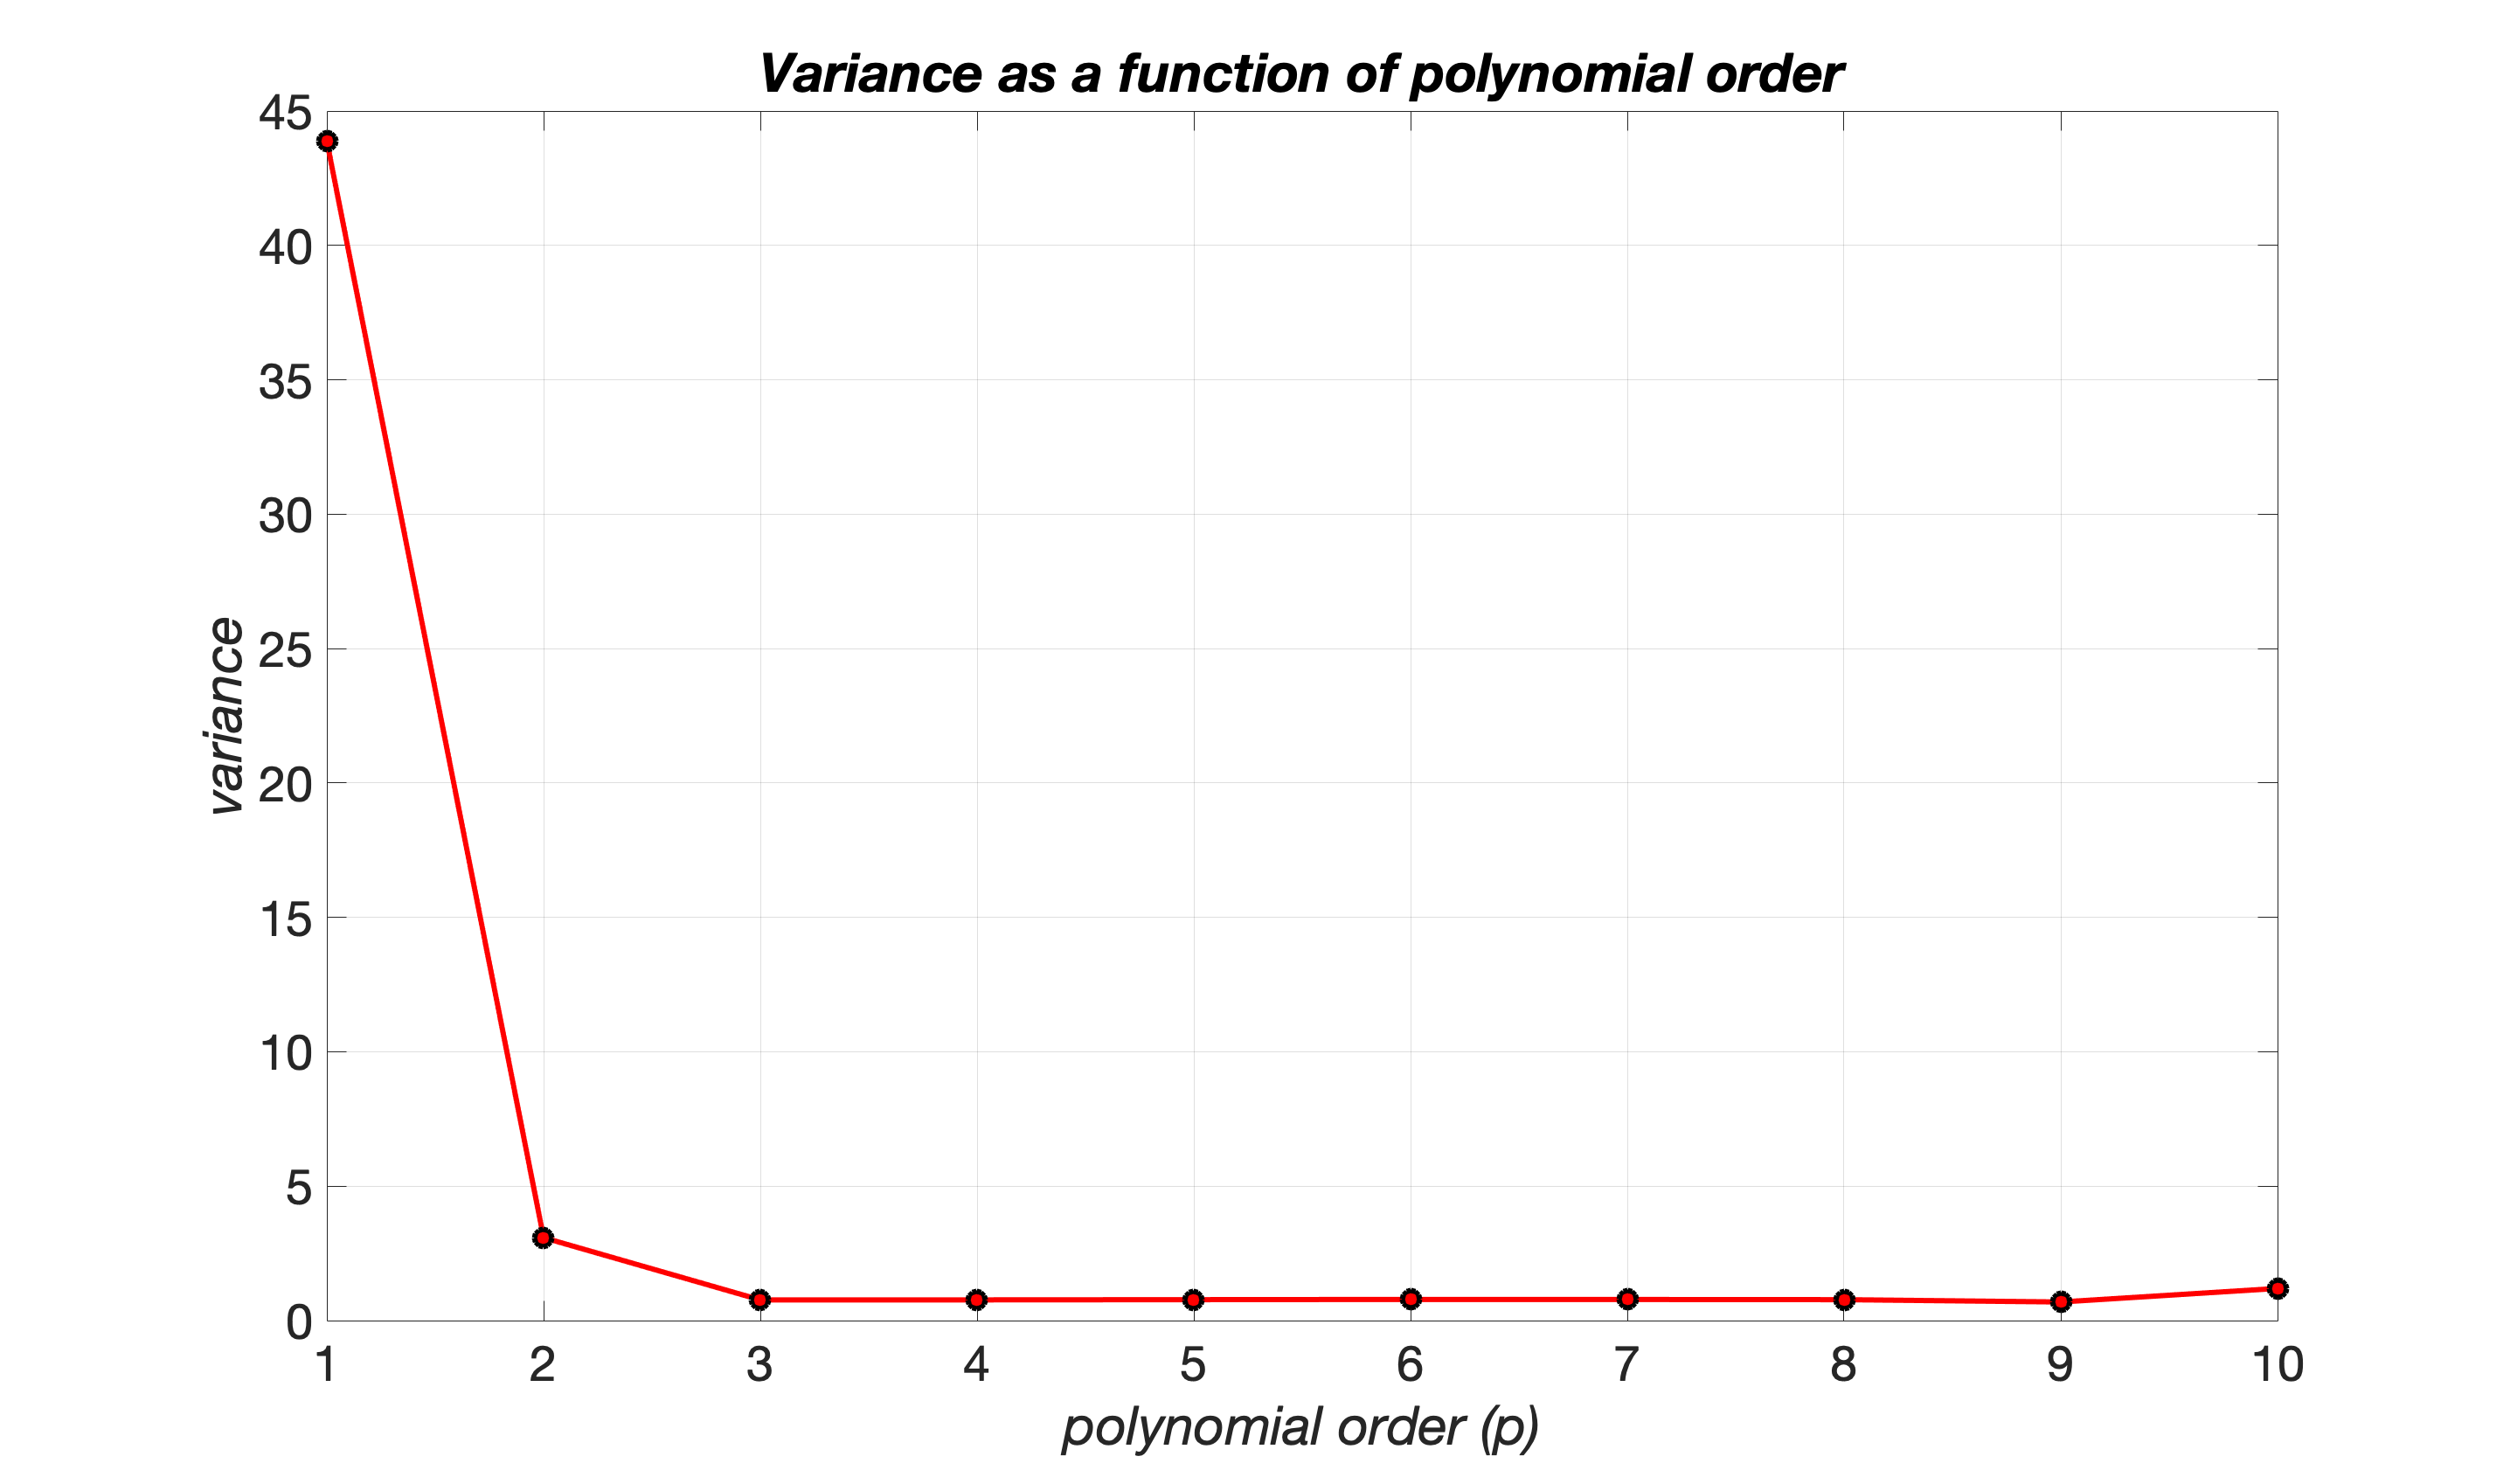
\includegraphics[scale=0.16]{ass4_1.png}}
\caption{Variance as a function of the polynomial order}
\label{Variance as a function of the polynomial order}
\end{figure}
\newpage
\noindent The output of the execution is shown below. The parameters for polynomial order 1 to 10 are printed and shown.
\begin{figure}[H]
\minipage{0.33\textwidth}
  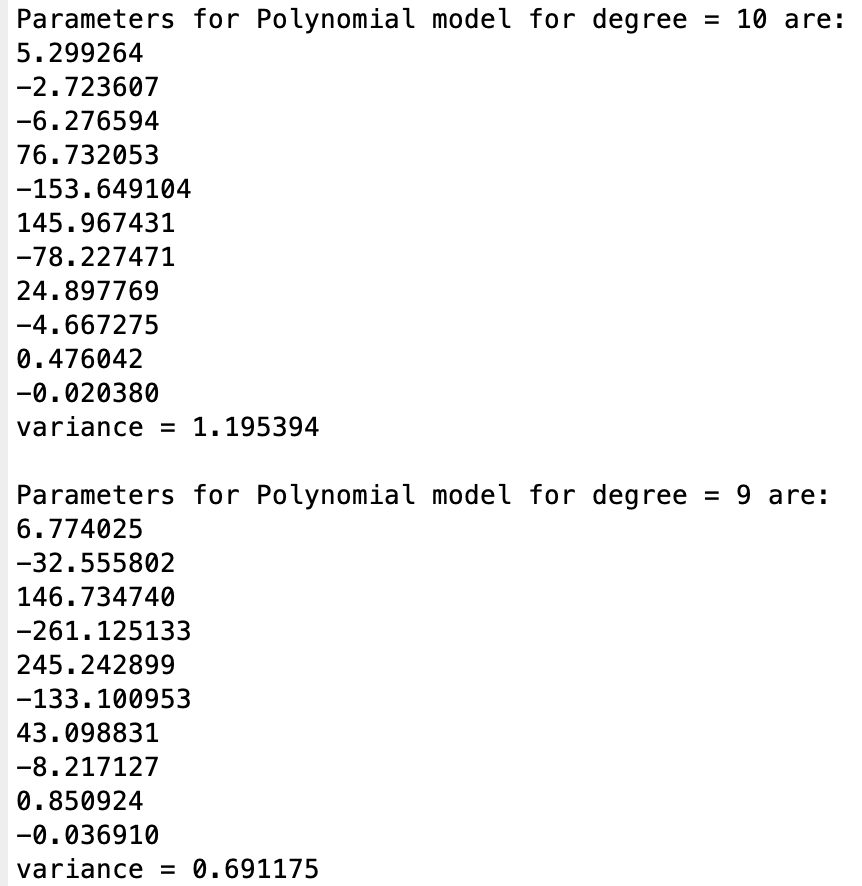
\includegraphics[width=\linewidth]{ass4_4.png}
\endminipage\hfill
\minipage{0.33\textwidth}
  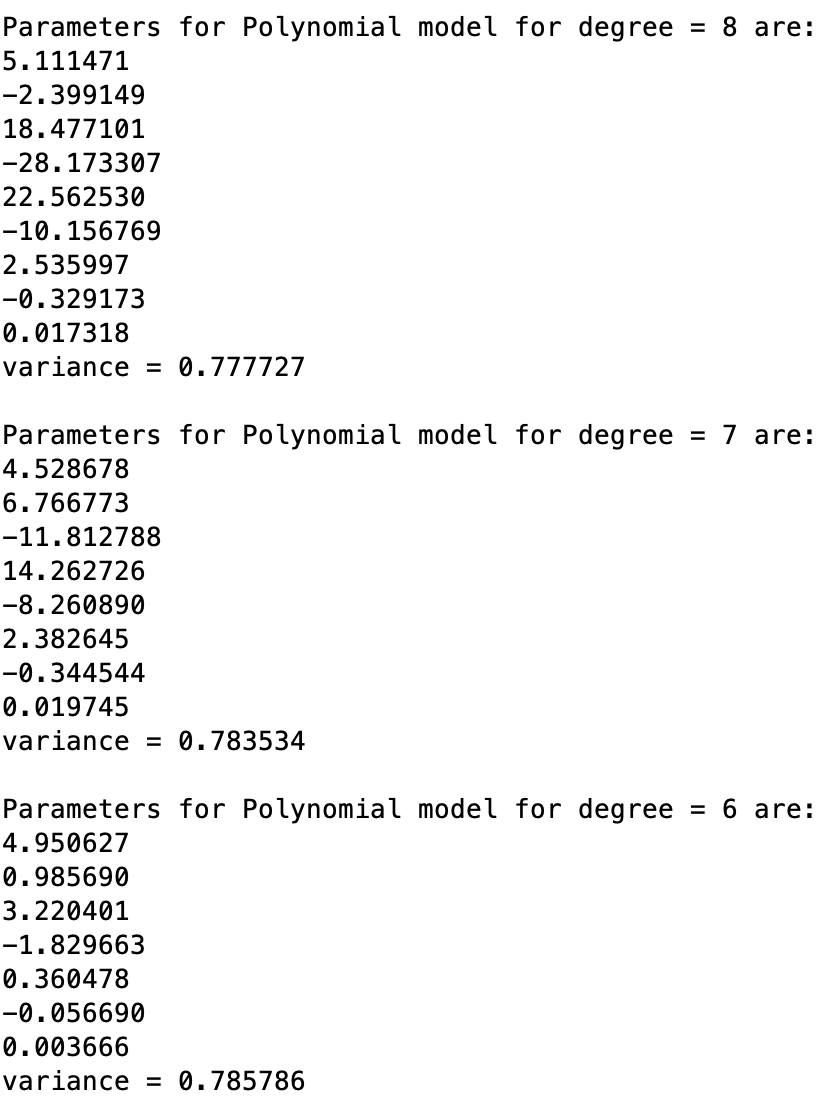
\includegraphics[width=\linewidth]{ass4_3.png}
\endminipage\hfill
\minipage{0.33\textwidth}%
  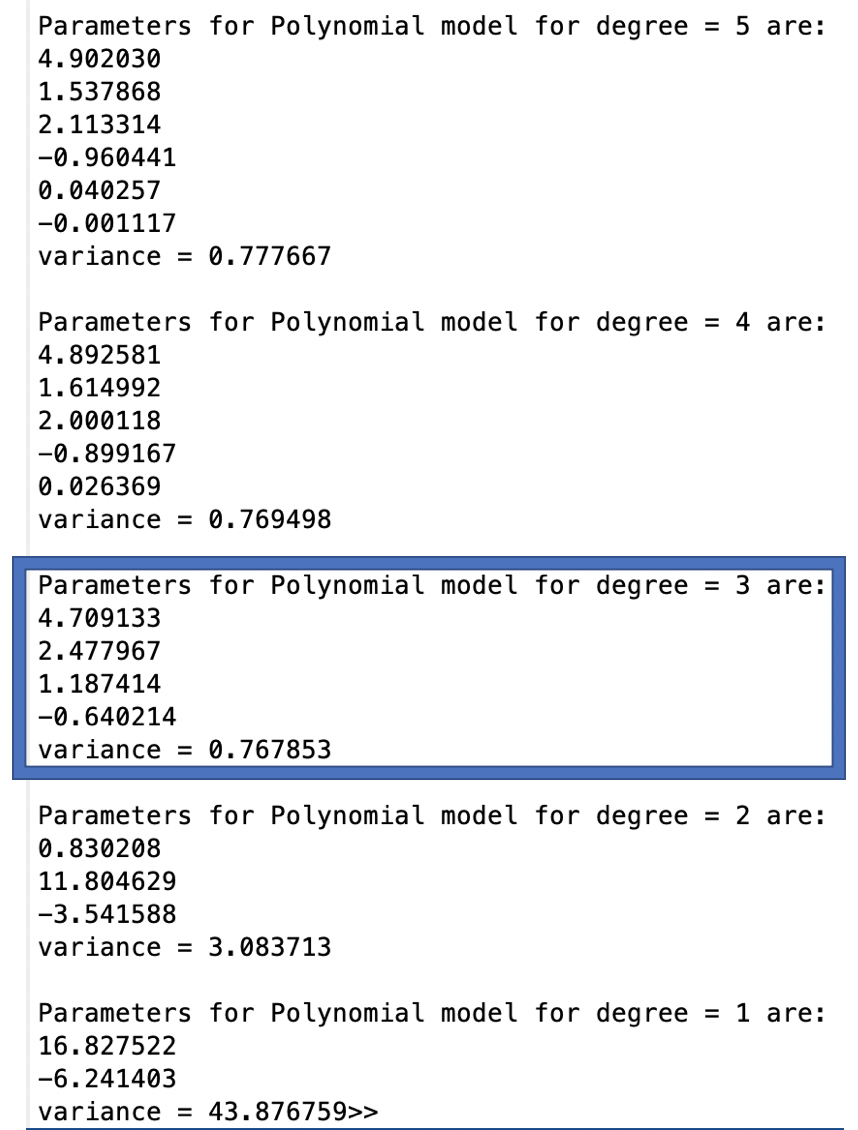
\includegraphics[width=\linewidth]{ass4_2.png}
\endminipage
\end{figure}

\noindent \textbf{Inference:} The variance reduces from 43.87 at $p = 1$ to 0.767 at $p = 3.$ Hence the polynomial of order 3 is considered to be the correct order. This is because, as the order increases further than 3, it remains almost constant. The parameters for the polynomial of order 3 are:  a = 4.77091, b = 2.47796, c = 1.187414 and d = -0.64021.
%%%%%%%%%%%  code 5  %%%%%

\section{Comparison of observations and estimated model}  \label{Comparison of observations and estimated model}
\noindent \textbf{Task:} For each of the models estimated above show the observations of the model ($x_i, y_i$) : $i = 1,2,...,N$ and the corresponding reconstructed model curve ($x_i, g(x_i)$) : $i = 1,2,...,N$ in one figure.
 
 \noindent \textbf{Solution:} We created a function \texttt{compare} inside the function \texttt{plotGraph} which used the values of the parameters from the previous exercise i.e., when $p = 3$ for polynomial model and $p = 1$ for the rest of the models to compare with the observed values from the data set which was previously created.\\
 
 \noindent \textbf{MATLAB code:}
\lstinputlisting{assignment3_5.m}

 \noindent \textbf{Output:}
 \noindent The output of the code is shown below. The estimated value is shown by a line while the observed value is represented by dots.
\begin{figure}[H]
    \centering
   \subfloat[Exponential model]{ {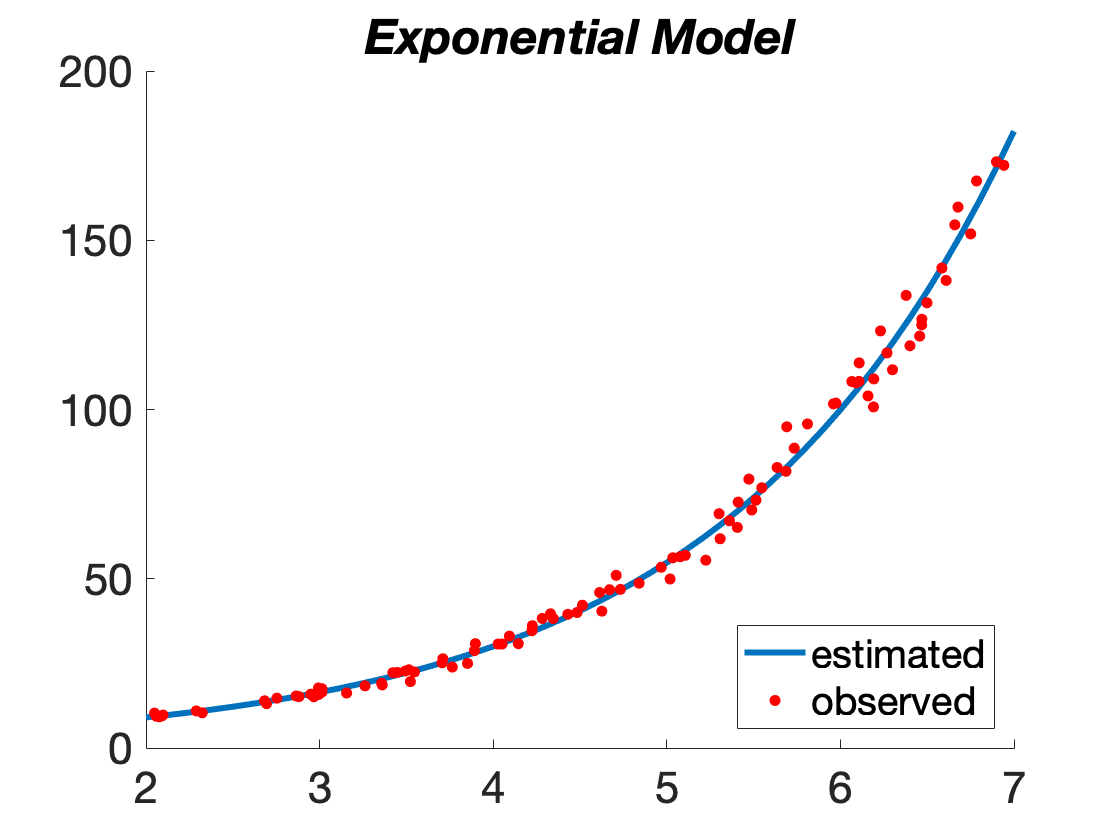
\includegraphics[width=7.6cm]{ass5_1.png}} }
    \qquad
    \subfloat[Sine model]{ {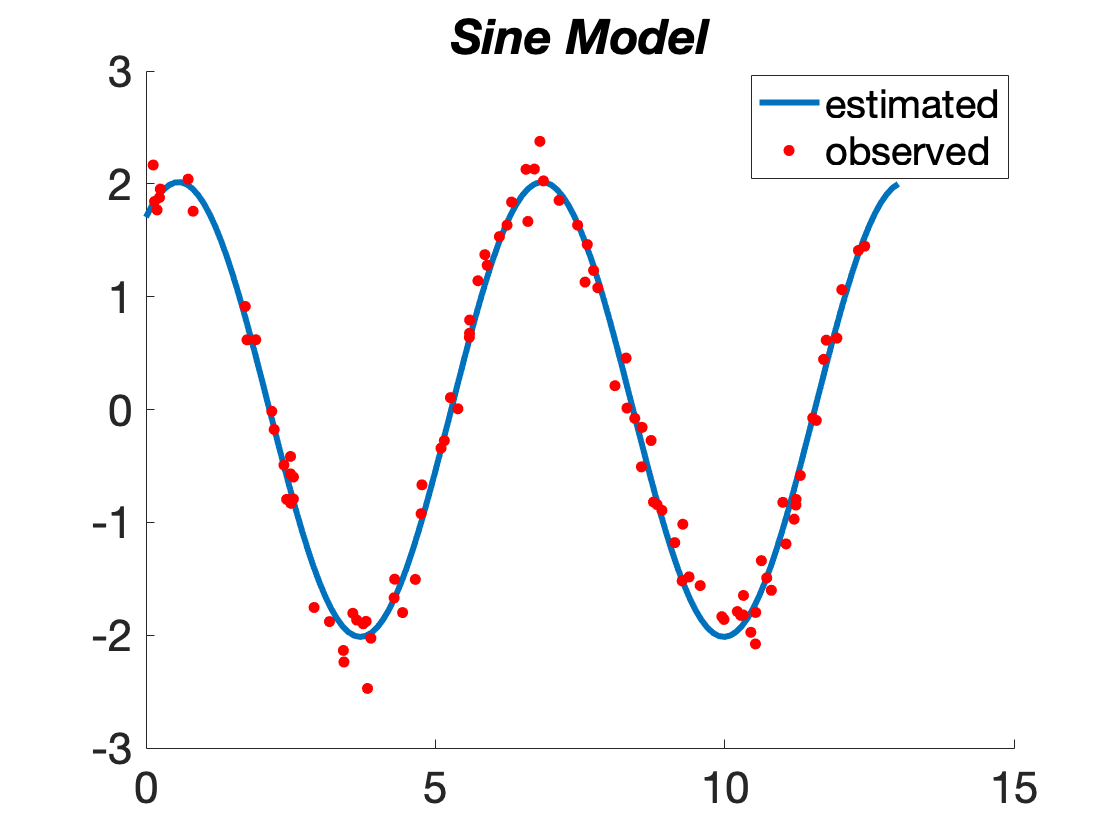
\includegraphics[width=7.6cm]{ass5_2.png} }}
\end{figure}
\begin{figure}[H]
    \centering
   \subfloat[Polynomial model]{ {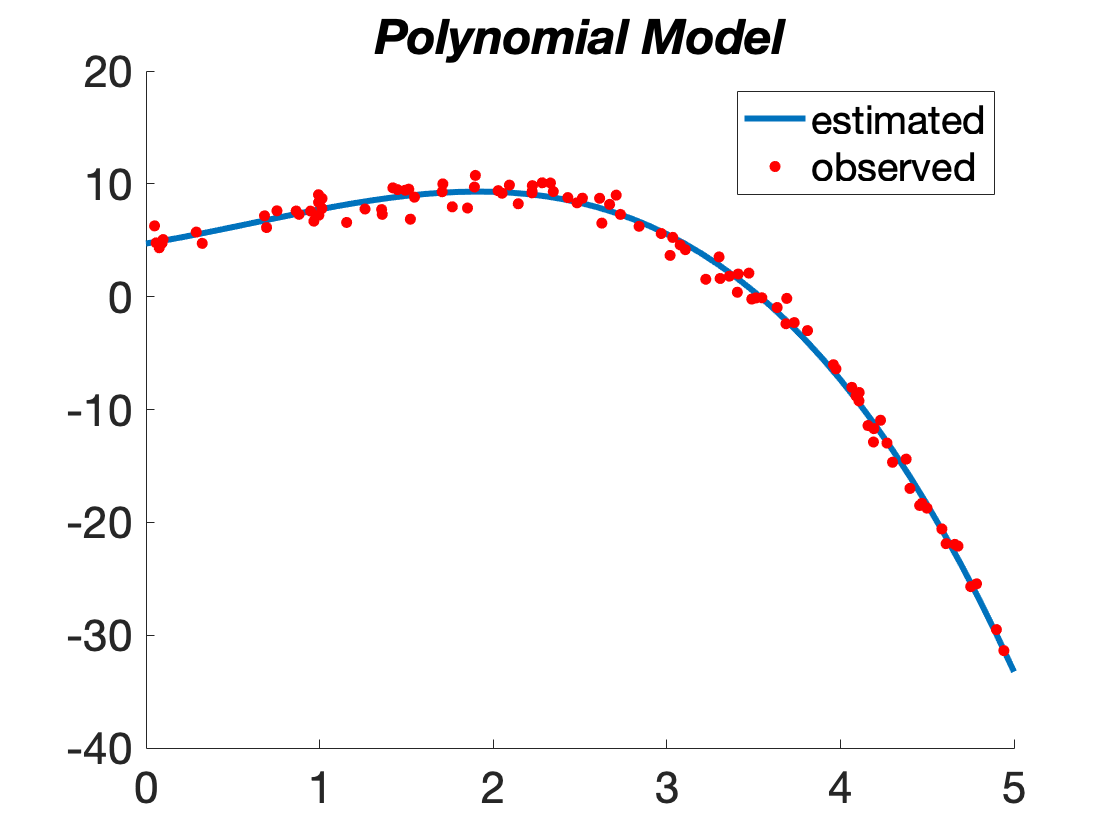
\includegraphics[width=7.6cm]{ass5_3.png}} }
    \qquad
    \subfloat[Power model]{ {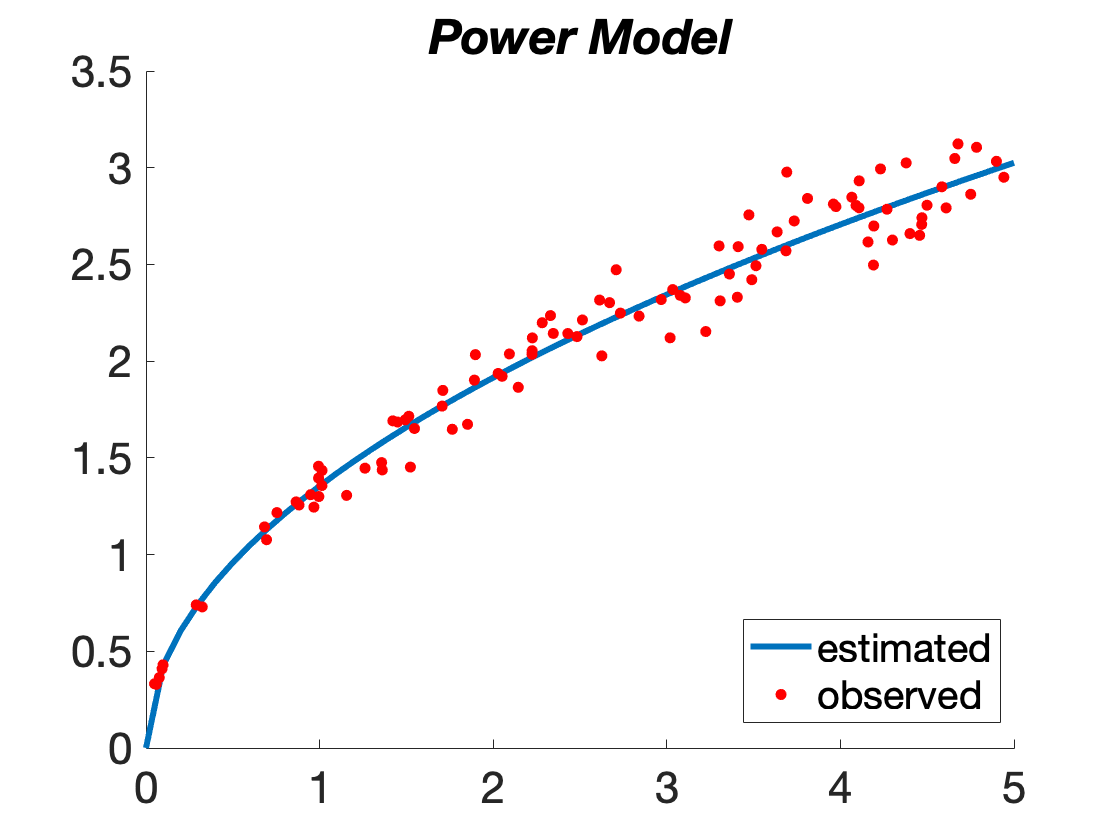
\includegraphics[width=7.6cm]{ass5_4.png} }}
    \caption{Comparison of observations and estimated models}
\end{figure}

\noindent \textbf{Inference:} We can infer that the observed value almost coincides with the estimated value. 

%%%%%% code 6 %%%%%%

\section{ LS-adjustment to a circle: estimating the centre  }  \label{ LS-adjustment to a circle: estimating the centre }
\noindent \textbf{Task:} Load \texttt{dat3\_2} containing a 100 $\times$ 2 matrix that represent the coordinates of 100 measurement points in the \textit{xy}-plane. Take a look at the measurement points and give from this the coordinates of the centre location. 


\noindent \textbf{Solution:} \texttt{dat3\_2} was loaded as mentioned in the task. It contains the matrix of data set $xy.$ We estimate and find the centre of the circle to be located at (4,2).\\ 
\noindent \textbf{MATLAB code:} 
\lstinputlisting{assignment3_6.m}
\newpage
\noindent \textbf{Output:} The output of the code is shown below. 
\begin{figure}[H]
\centering
{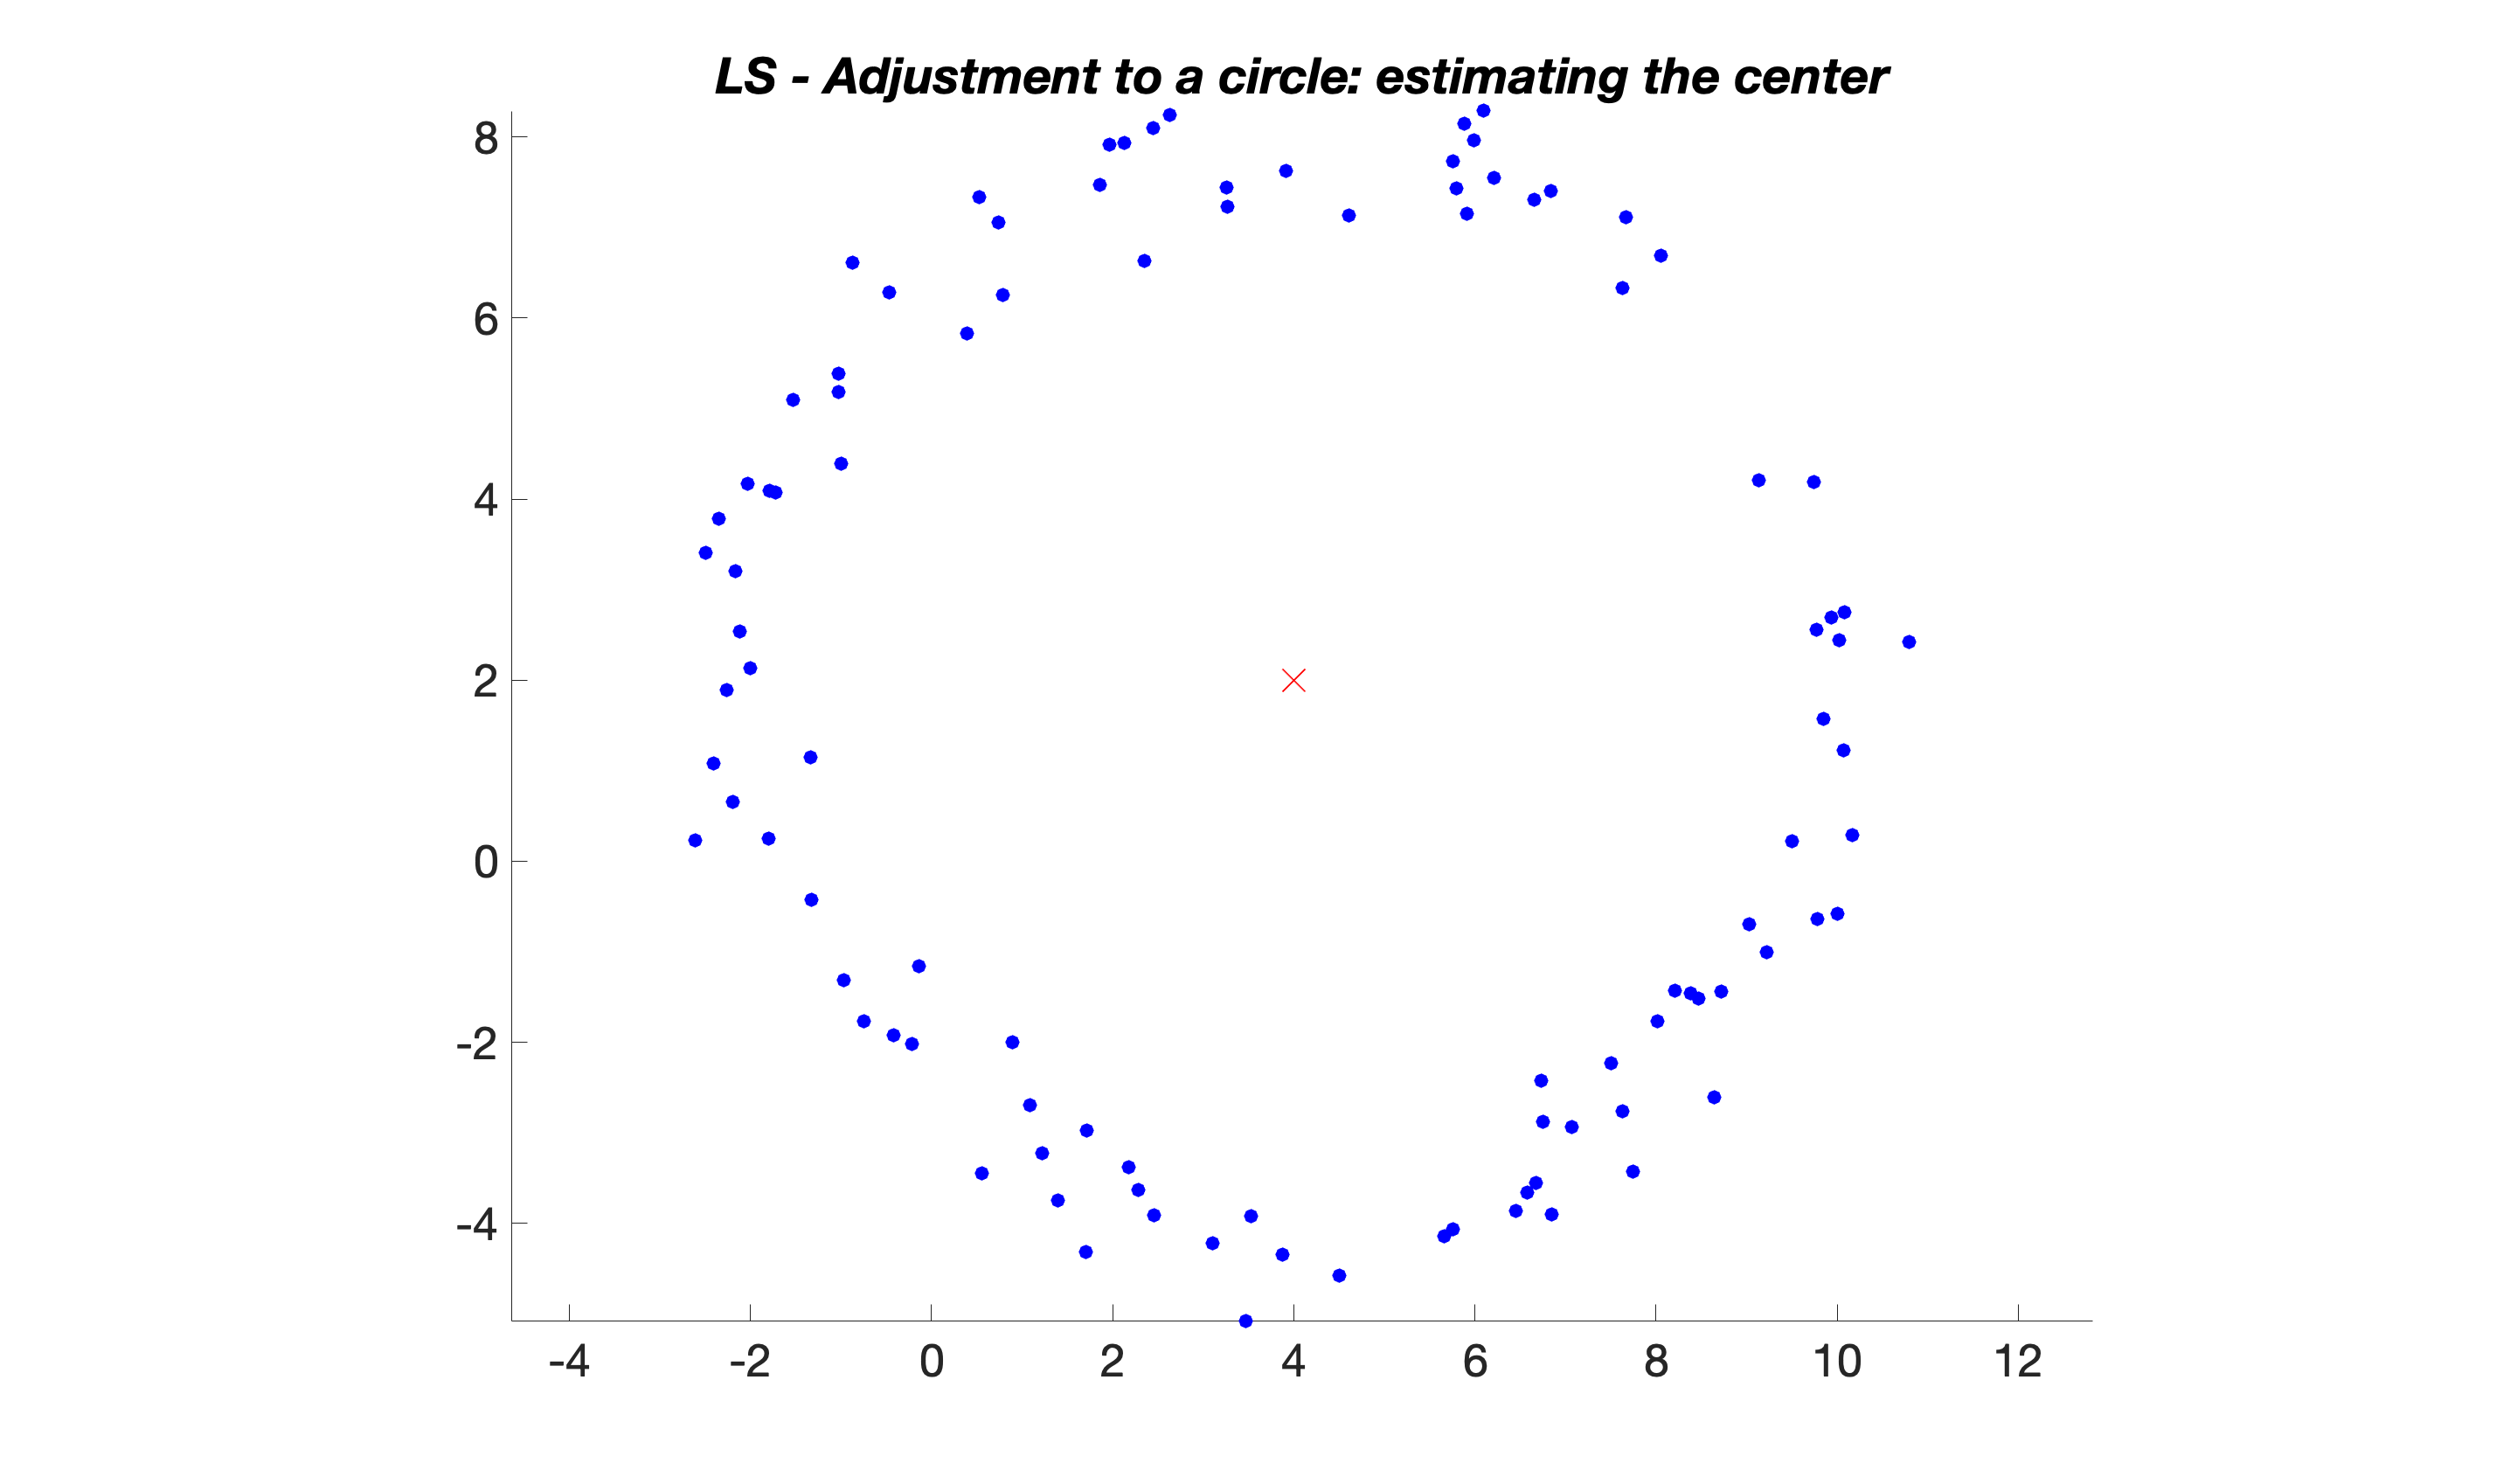
\includegraphics[scale=0.15]{ass6_1.png}}
\caption{LS-adjustment to a circle: estimating the centre }
\label{LS-adjustment to a circle: estimating the centre }
\end{figure}

\noindent \textbf{Inference:} The measurement points nearly takes the shape of a circle with centre at (4,2)


%%%%%% code 7 %%%%%%

\section{ LS-Fit to a circle: iteration }  \label{ LS-Fit to a circle: iteration }
\noindent \textbf{Task:} Carry out a LS-Estimation as shown in section 3.1.5. Use the estimated centre as an improved initial value and repeat the LS-Estimation as long as $ ||(\tilde{X_0}(k), \tilde{Y_0}(k)) - (\tilde{X_0}(k-1), \tilde{Y_0}(k-1))|| < 10^{-10} $ is fulfilled, where $ (\tilde{X_0}(k), \tilde{Y_0}(k)) $ denotes the \textit{k}-th LS-Estimate of the centre. Write a function \texttt{LSE\_circle} that carries out the iteration. Depict the reconstructed circle and the measurement points in a diagram.


\noindent \textbf{Solution:} We carry a linear LS - Approach to a circle which is mentioned in topic 1.5. We wrote a function \texttt{LSE\_circle} which outputs the LS-estimated circle fitting when given the measured points as the input. Maximum iteration time is added to control the termination incase the code does not converge.\\
\noindent \textbf{MATLAB function \texttt{LSE}:}
\lstinputlisting{LSE_circle.m}

\noindent \textbf{MATLAB code:} 
\lstinputlisting{assignment3_7.m}

\noindent \textbf{Output:} The output of the code is shown below. 
\begin{figure}[H]
\centering
{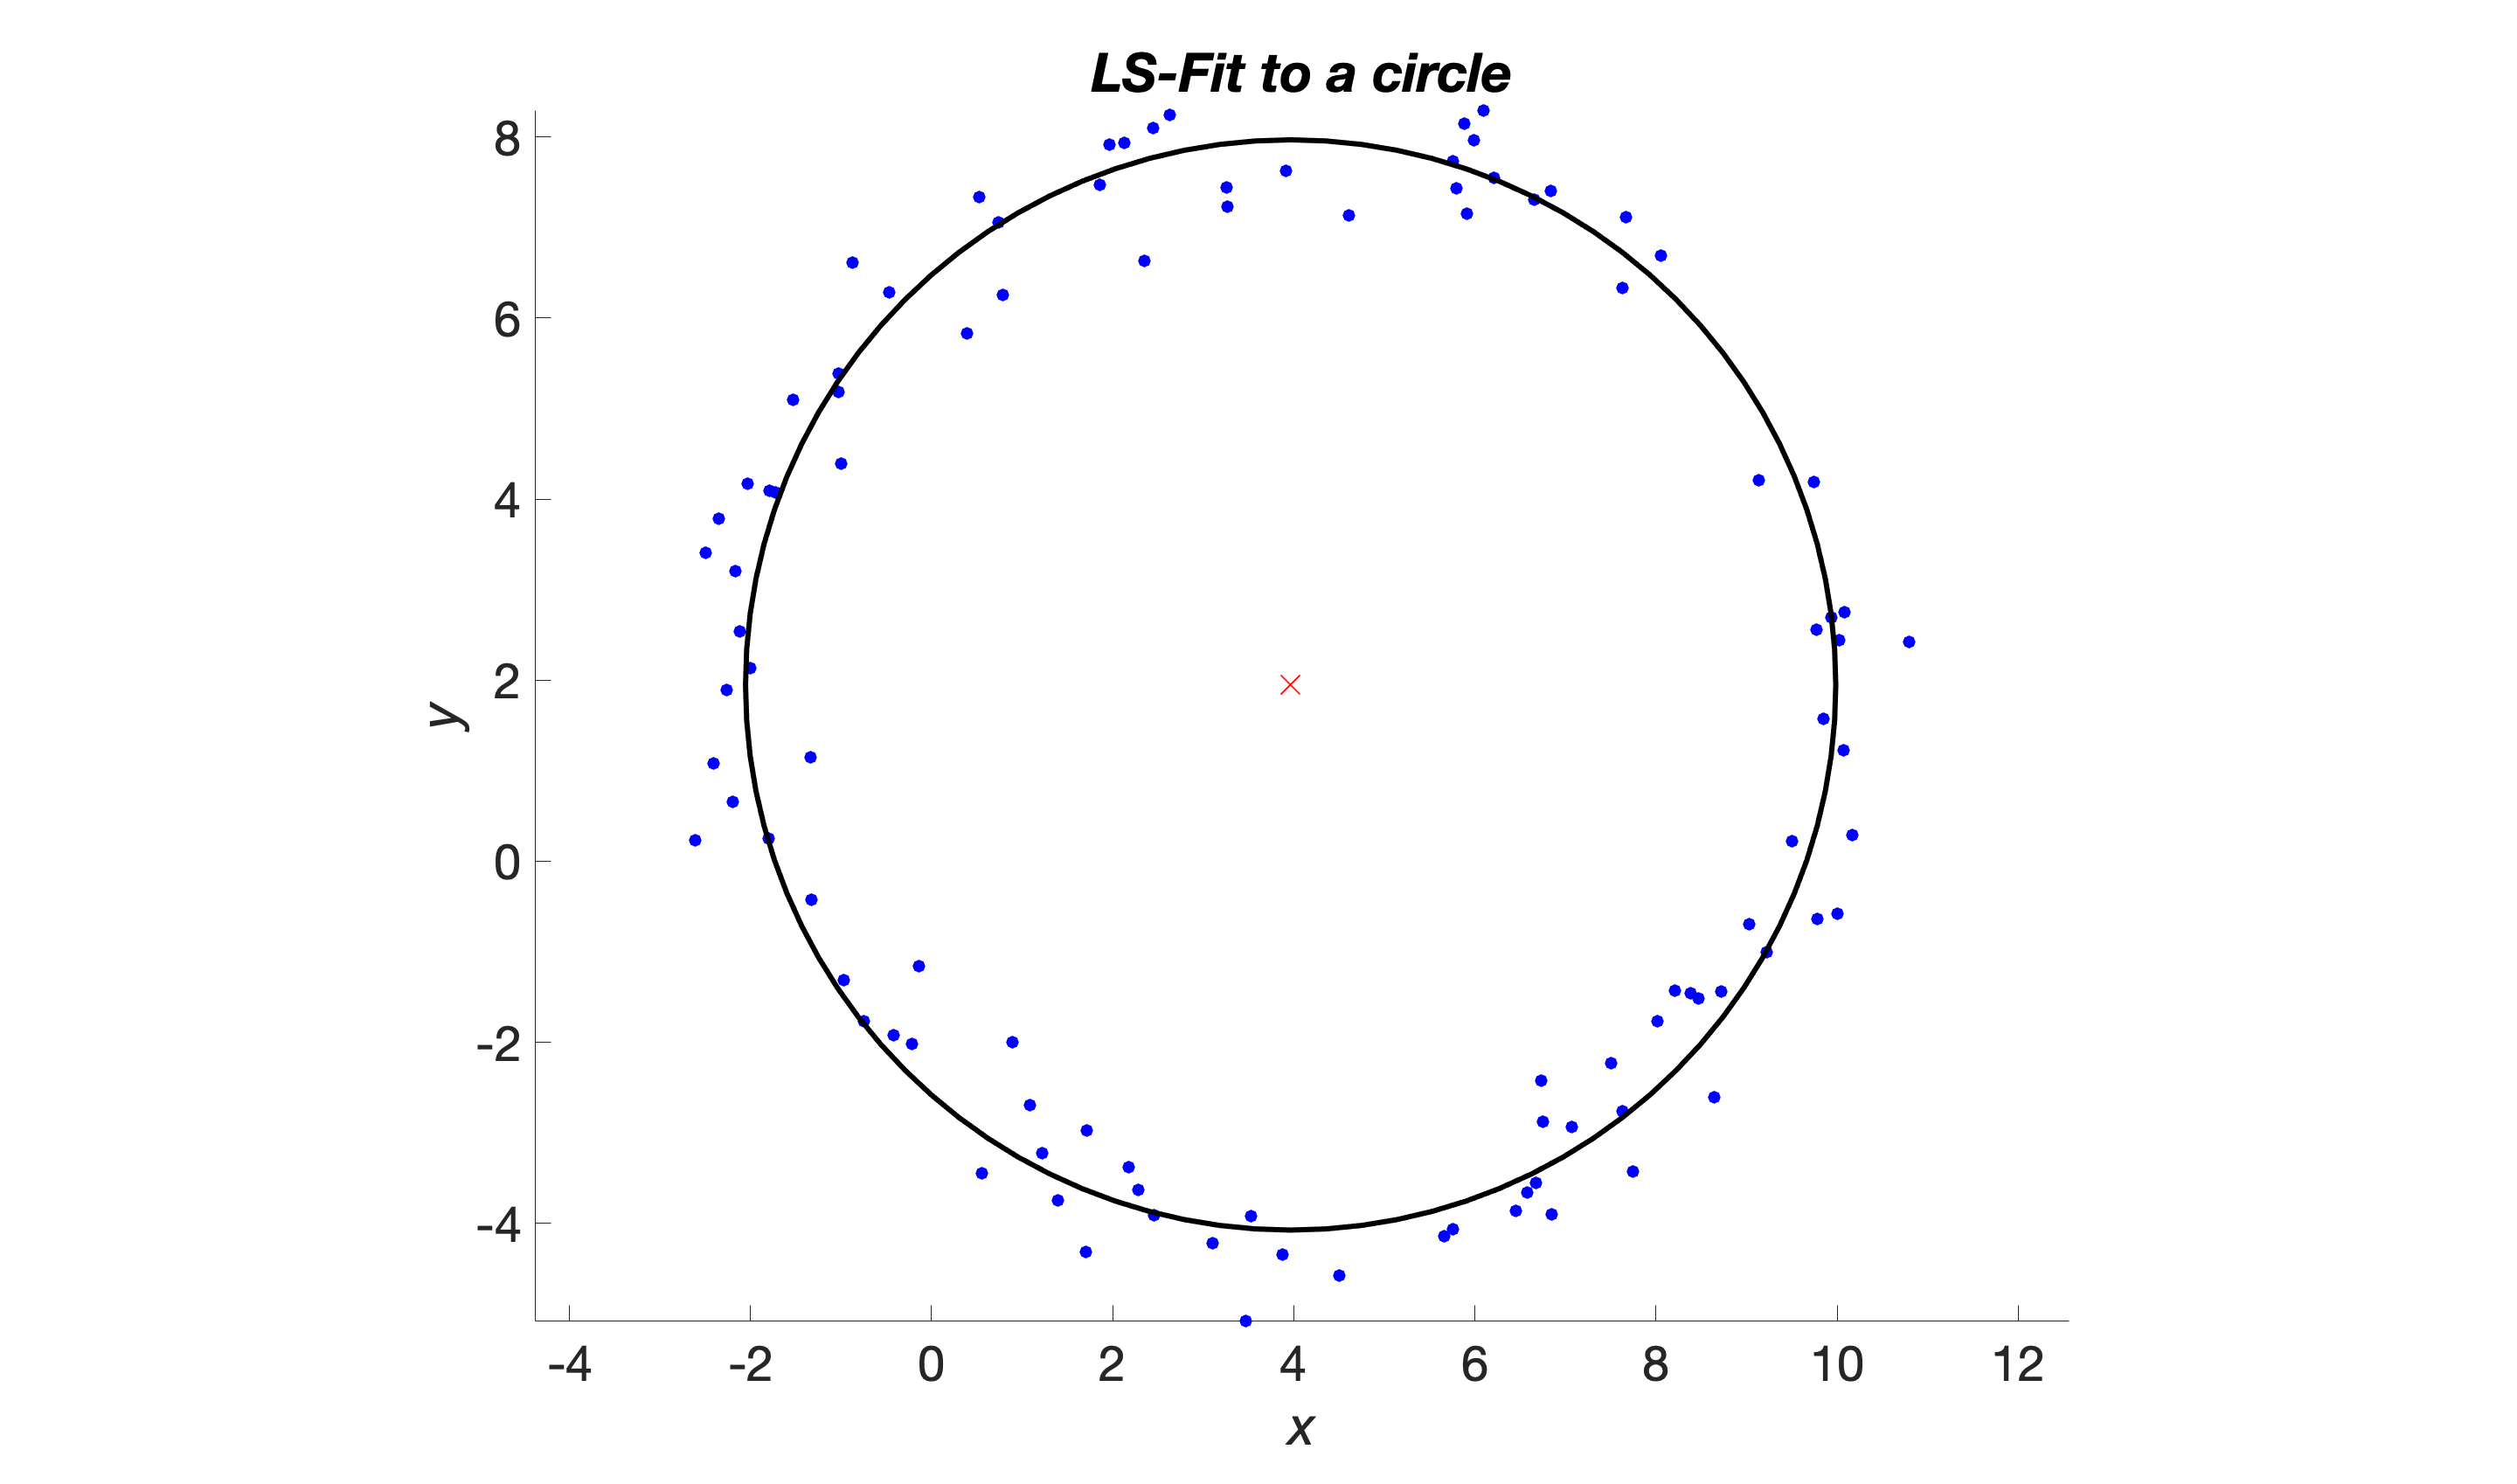
\includegraphics[scale=0.13]{ass7_1.png}}
\caption{LS-Fit to a circle: iteration }
\label{LS-Fit to a circle: iteration }
\end{figure}

\noindent The execution of the code gives us the following result.
\begin{figure}[H]
\centering
{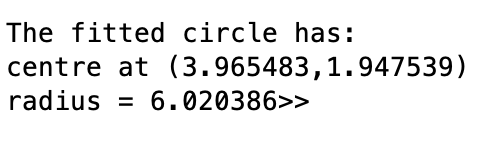
\includegraphics[scale=0.75]{ass7_2.png}}
\end{figure}
\noindent \textbf{Inference:} The measurement points nearly takes the shape of a circle with centre at (3.965,1.947) and radius of 6.020.


%%%%%% code 8 %%%%%%

\section{ LLS-Fit to a circle: convergence}  \label{ LS-Fit to a circle: convergence }
\noindent \textbf{Task:} Does this method converge, if the initial guess of the circle center is very poor? Try it by giving your function \texttt{LSE\_circle} intentionally a very poor initial estimate of the centre location. Explain your observation.\\

\noindent \textbf{Solution:} The function \texttt{LSE\_circle} mentioned earlier is used again in this program. In this method, we require an initial guess of the centre of the circle. If this guess is poor, the method does not converge and no result can be obtained.\\
\noindent \textbf{MATLAB code:} 
\lstinputlisting{assignment3_8.m}

\noindent \textbf{Output:} The output of the code is shown below. The blue dots represent convergence while the red represent non convergence. Thus, taking the blue points as initial guess will lead to convergence and vice versa.
\begin{figure}[H]
\centering
{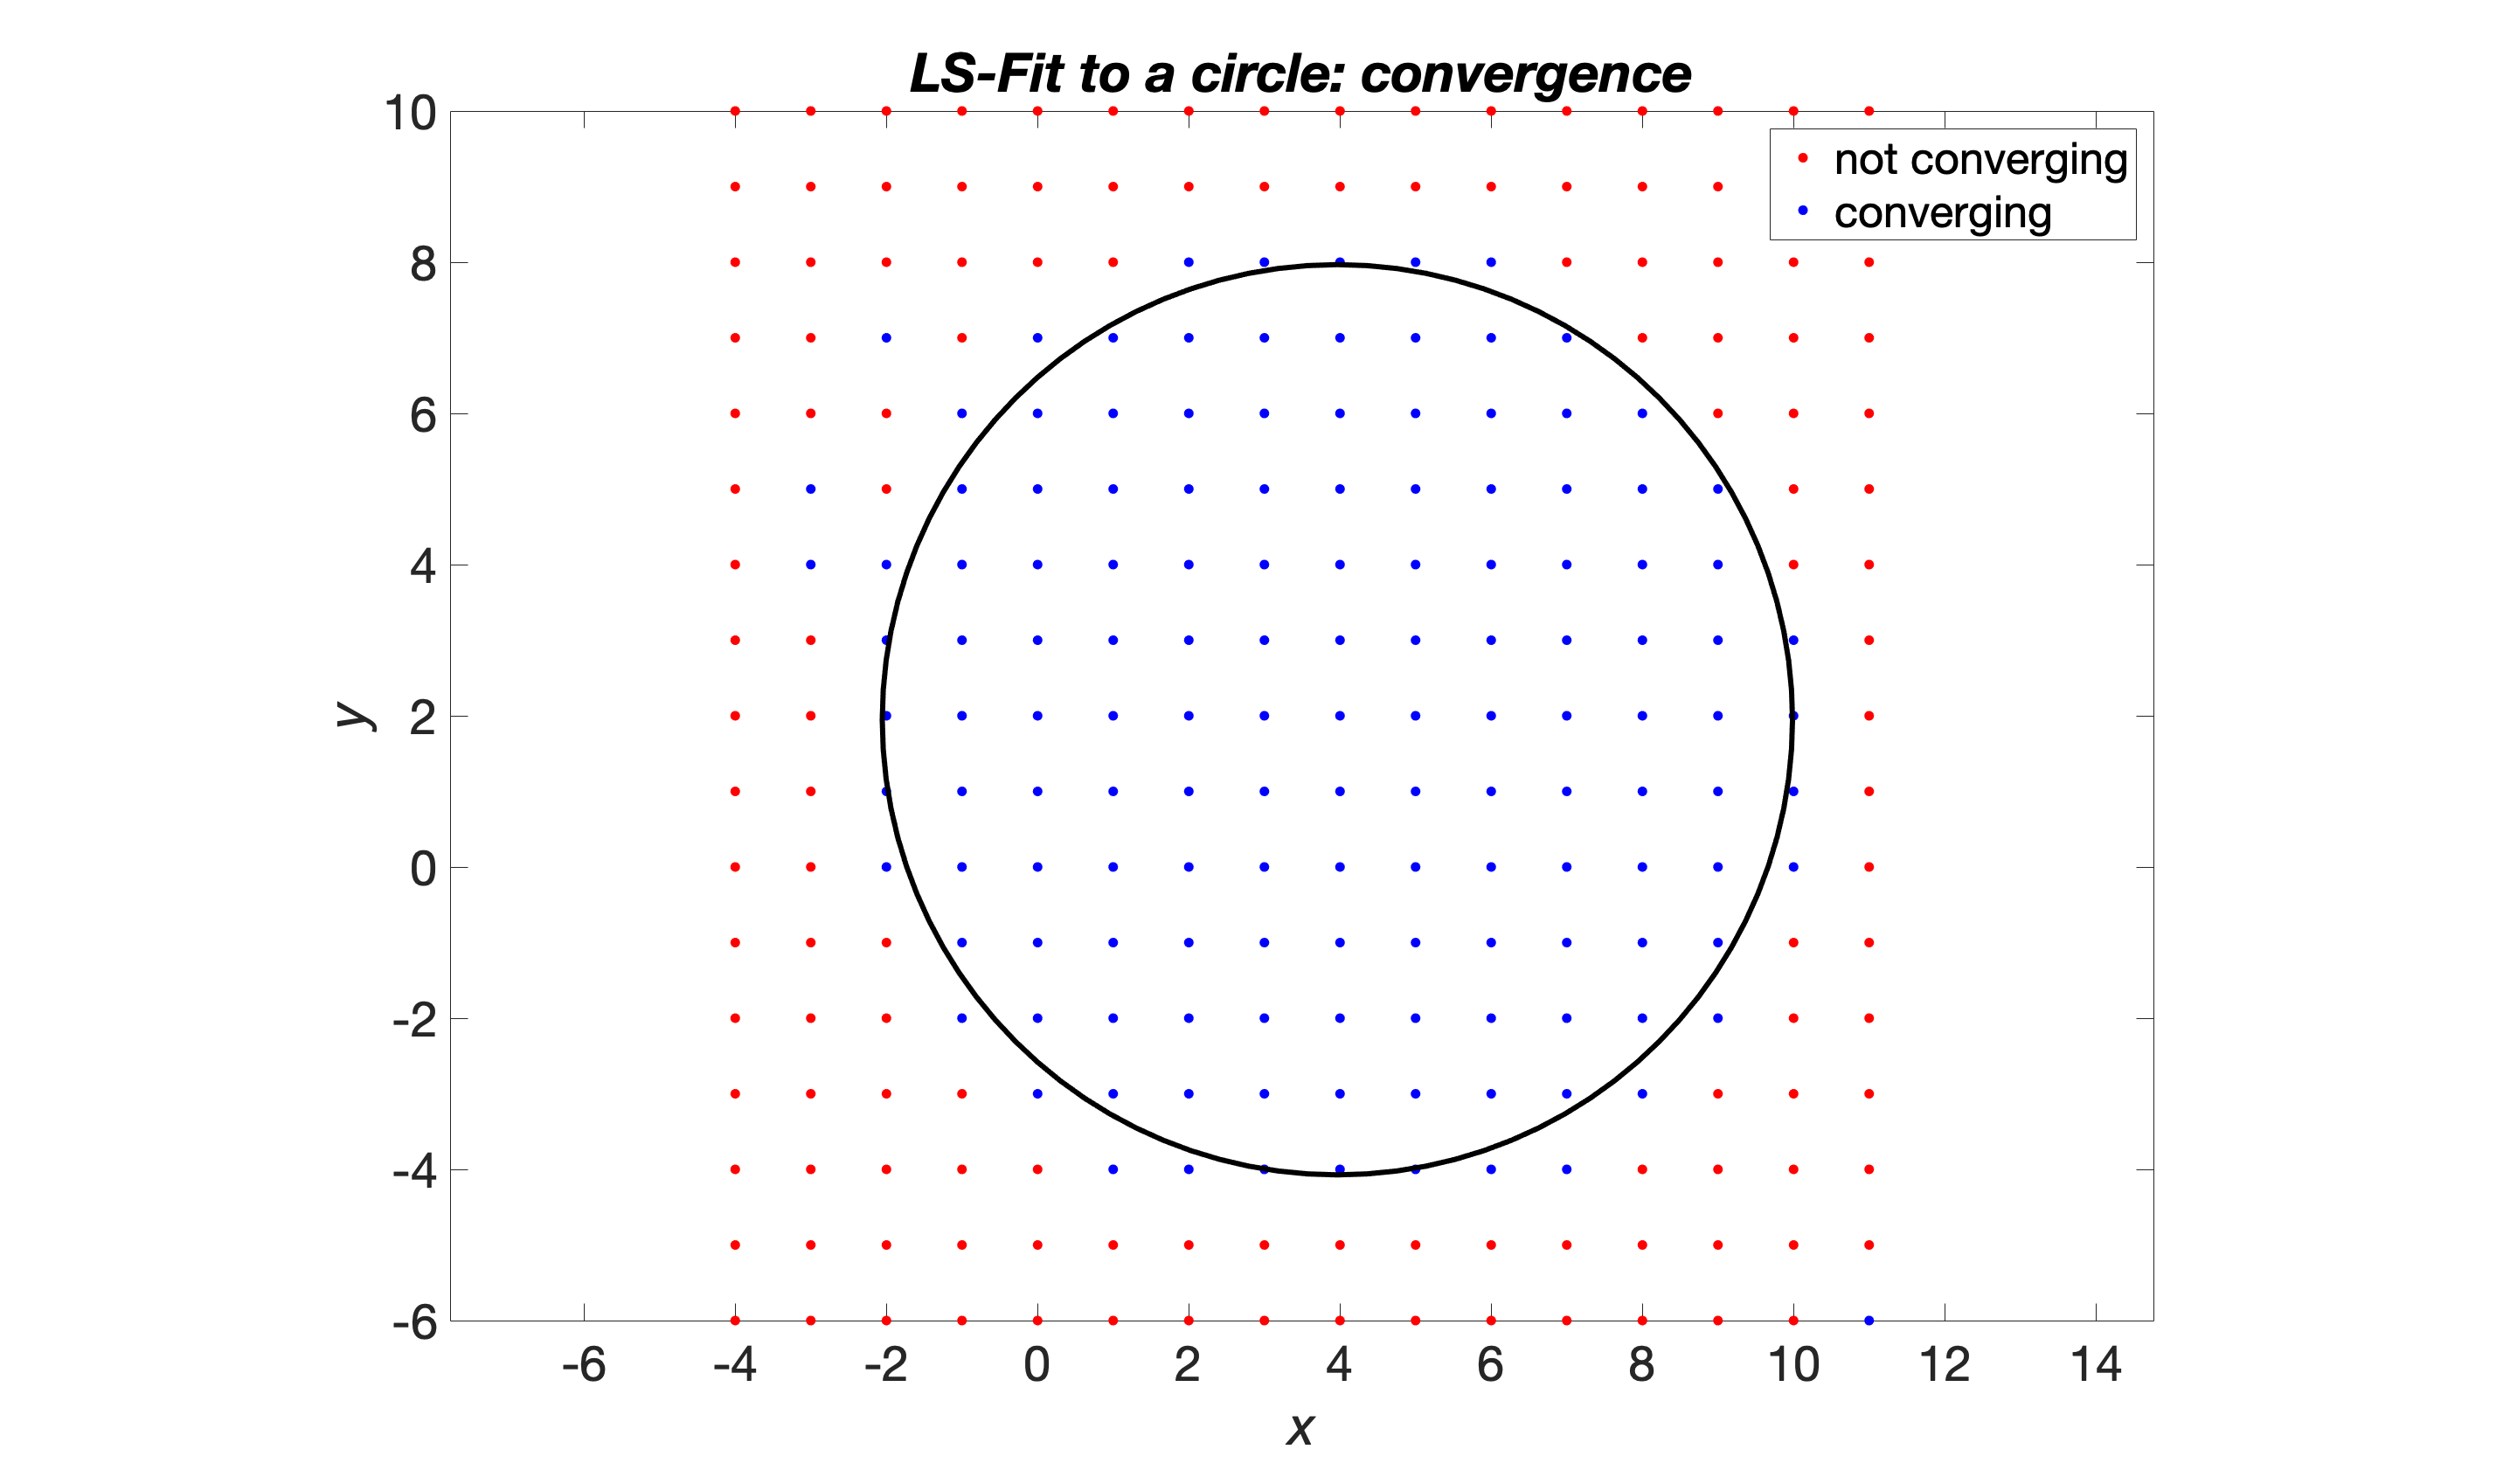
\includegraphics[scale=0.15]{ass8_1.png}}
\caption{LS-Fit to a circle: convergence }
\label{LS-Fit to a circle: convergence }
\end{figure}

\noindent \textbf{Inference:} Majority of the blue dots lie inside the circle leading to convergence. Few blue dots lie outside the circle which can also allow convergence. If the initial guess is placed where there is a red dot, the system will not converge and hence no result will be obtained.